\documentclass[border=5pt]{standalone}
\usepackage{tikz}
\usetikzlibrary{calc}
\usepackage{amsmath}
\begin{document}
    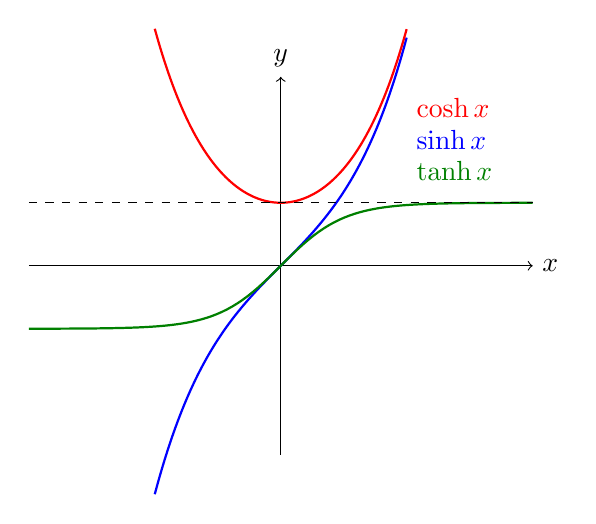
\begin{tikzpicture}[scale=0.8]
        % Axes
        \draw[->] (-4,0) -- (4,0) node[right] {$x$};
        \draw[->] (0,-3) -- (0,3) node[above] {$y$};

        % sinh(x)
        \draw[blue, thick, domain=-2:2, samples=100]
            plot (\x, {(exp(\x) - exp(-\x))/2});
        \node[blue, right] at (2,2) {$\sinh x$};

        % cosh(x)
        \draw[red, thick, domain=-2:2, samples=100]
            plot (\x, {(exp(\x) + exp(-\x))/2});
        \node[red, right] at (2,2.5) {$\cosh x$};

        % tanh(x)
        \draw[green!50!black, thick, domain=-4:4, samples=100]
            plot (\x, {(exp(\x) - exp(-\x))/(exp(\x) + exp(-\x))});
        \node[green!50!black, right] at (2,1.5) {$\tanh x$};

        % Asymptote y=1 for cosh
        \draw[dashed] (-4,1) -- (4,1);
    \end{tikzpicture}
\end{document}
